%%report template for pattern recognition SS2016

\documentclass[english, paper=a4]{scrartcl}
\usepackage[utf8]{inputenc}
% images
\usepackage{graphicx}
%math
\usepackage{amsmath,amssymb}
%code
\usepackage{algorithm}
\usepackage[noend]{algpseudocode}
\makeatletter
\def\BState{\State\hskip-\ALG@thistlm}
\makeatother

\usepackage{subcaption}
\captionsetup{compatibility=false}
\usepackage{multirow}
\usepackage{color}
\usepackage{enumitem}


\begin{document}

\graphicspath{{images/}}


%%------------------------------------------------------
%% provide your input here:
\title{Assignment 1 - Page Detection} 

\subtitle{Document Analysis} 

\author{Timon Höbert(01427936) \\ Manuel Mayerhofer (01328948)\\ Stefan Stappen(01329020)}



%%------------------------------------------------------

\maketitle


%%------------------------------------------------------

\section{Definition of Task}
Page detection is the task of detecting and segmenting the page outline of a document within an image. The ICDAR2015Competition on Smartphone Document Capture and OCR (SmartDoc) \cite{burie2015icdar2015} is the first competition for document page detection and Smartphone OCR. The first assignment is the page detection.\\
The input is a set of video clips containing a document at different backgrounds. The output contains the bounding box of the document in quadrilateral coordinates per each frame of the video clip.

\section{Dataset}
The dataset consists of six different document types: Datasheet, letter, magazine, paper, patent, and tax.
For each document type, there are five different documents, which cover different document layout schemes and contents.
The six document types are recorded on five different backgrounds. A result is a number of 30 videos per background and a total of 150 videos. The videos are recorded using FULL HD resolution at variable frame rate.  
Every video has a duration of around 10 seconds. The videos include distortions like focus and motion blur, the perspective of the document, change of illumination and partial occlusions of the document pages. Each frame is ground-truthed by annotating the quadrilateral coordinates of each frame in an XML file.

\section{Implementation}
Our method is based on the method of P Li, Y Niw and X. Li from NetEase.



\subsection{Line Segment Detector}
After the preprocessing we use the line segment detector (LSD) \cite{von2010lsd} to detect the lines in the image. We use the LSD-OpenCV-MATLAB \cite{lsd2014}.The line of the LSD algorithm is shown in Figure \ref{fig:lsd}

\begin{figure}[h]
\centering
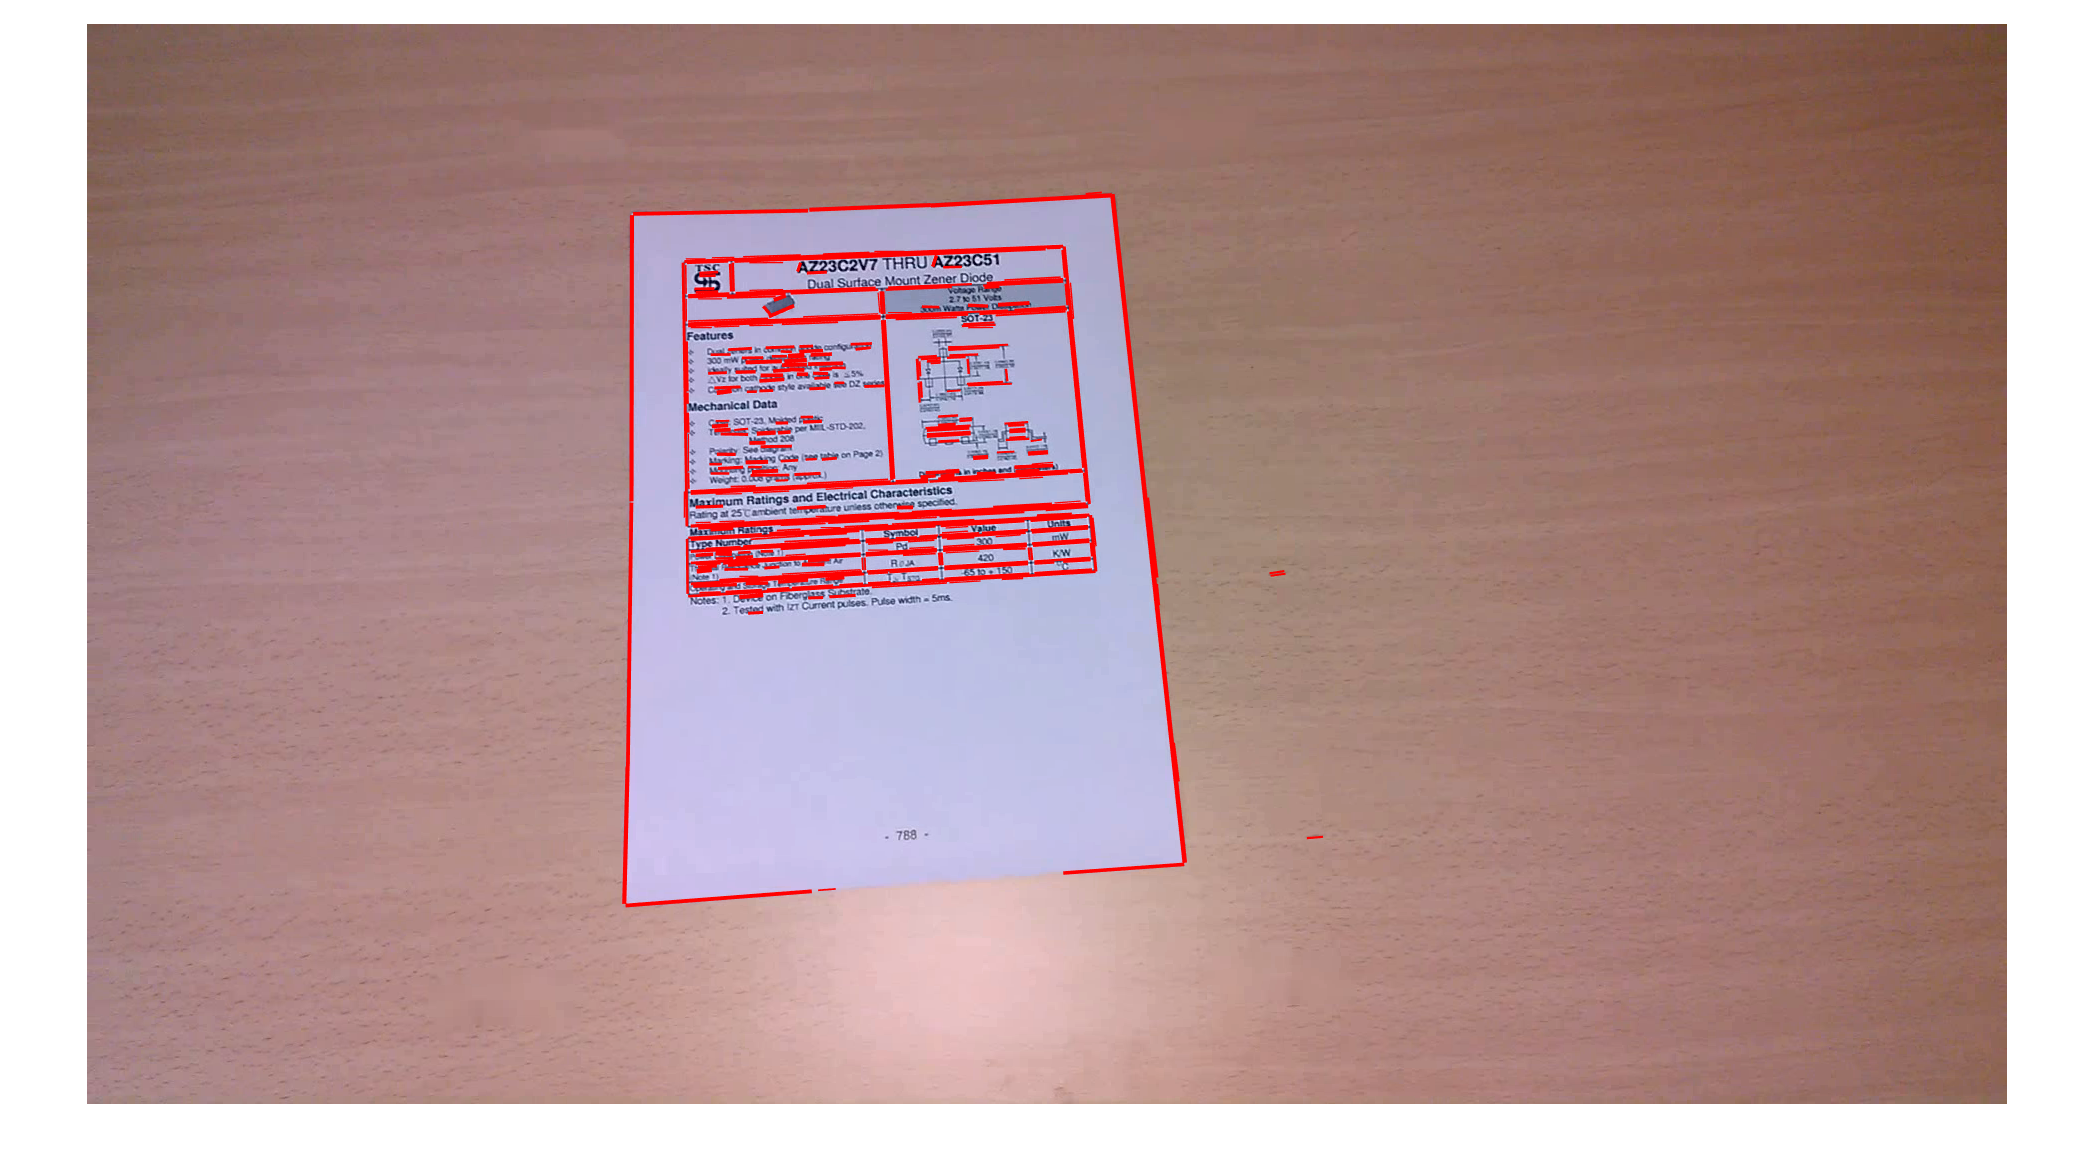
\includegraphics[width=0.7\textwidth]{lsd.png}
\caption{Red lines from the LSD algorithm.}
\label{fig:lsd}
\end{figure}

The LSD algorithm detects the essential lines in the image, but many lines are very short. Some lines segments represent one line, so we have to merge it. The founded set of lines is reduced as follows. Lines are removed which have a minimum length of the image size. Furthermore, lines are removed which are near the border of the image or which have their starting point on the border of the image.\\
The line segments are grouped in horizontal and vertical segments. After that, we merge lines that have the same direction with a certain margin between the line segments.
The result of the reduced merged set of lines is shown in Figure \ref{fig:redLines}.

\begin{figure}[h]
\centering
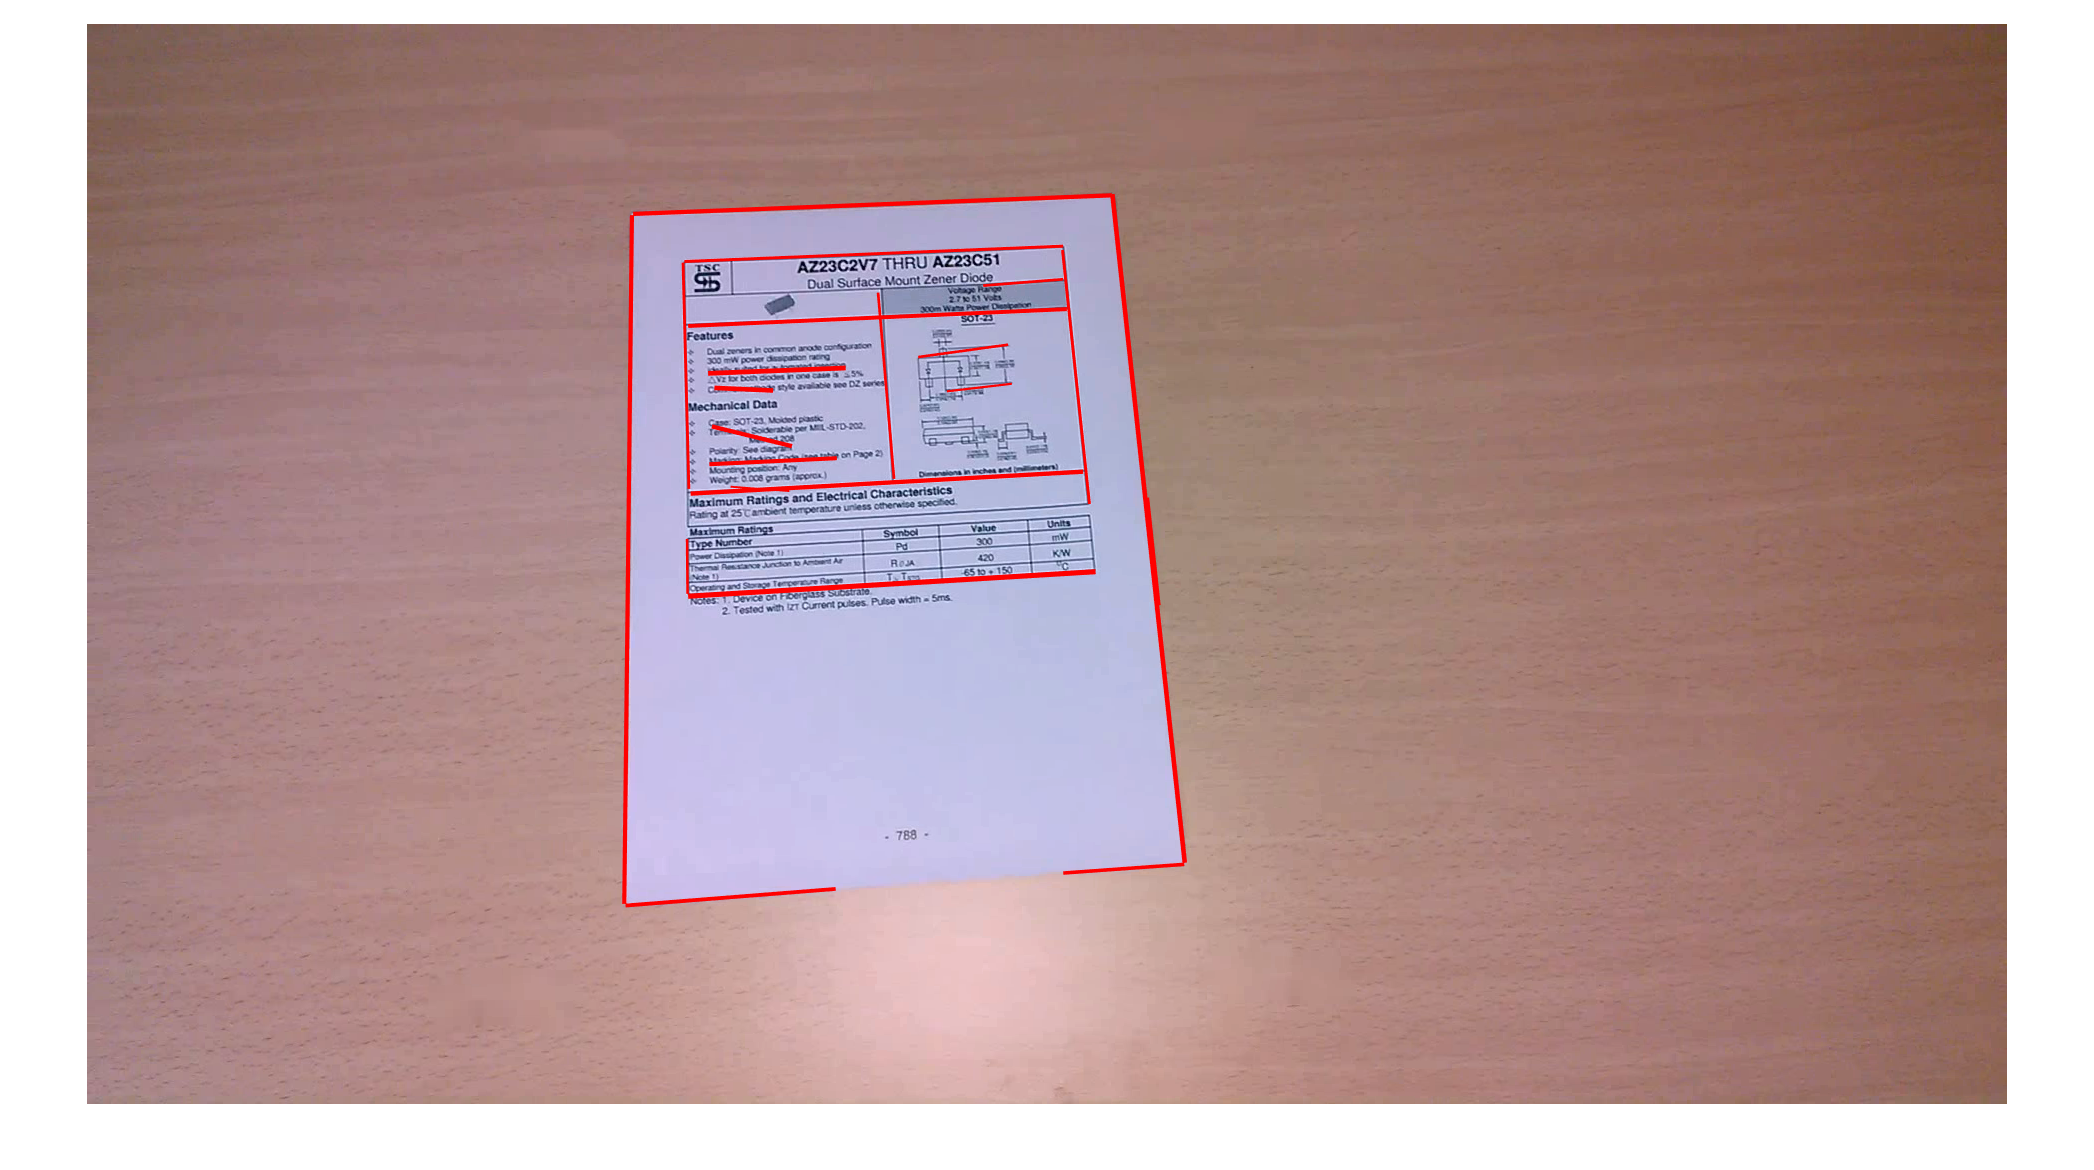
\includegraphics[width=0.7\textwidth]{redLines.png}
\caption{Reduced set of lines.}
\label{fig:lsd}
\end{figure}

\subsection{Bounding Box Calculation}
Then we select two horizontal and two vertical lines and check if both horizontal lines have smaller x coordinates or higher x coordinates as the minimum or maximum x coordinate of the vertical line to check if the line matching make sense. We do the same for vertical lines with the y coordinate. First we select only lines that have at least 3 of 4 similar start, or end points. Then we calculate the bounding boxes of the document.

\subsection{Best Bounding Box Selection}
For every bounding box we calculate the following properties:
\begin{itemize}
\item Area
\begin{itemize}
\item The area is the most important property because we choose the bounding box with the greatest area, but we also check if the area exceeds a limit because sometimes the table is also recognized and this would form the greatest area. 
\end{itemize}
\item Length of the horizontal and vertical lines
\begin{itemize}
\item We check if the two horizontal lines are equal in length with a little threshold, for vertical lines respectively. 
\end{itemize}
\item Aspect ratio
\begin{itemize}
\item We assume that we recognize documents in the A4 format in portrait format or horizontal format.
\end{itemize}
\item Inner angles
\begin{itemize}
\item We check if the inner equals are similar to 90 degrees, but because of the perspective distortion, we accept a high deviation of the angles to achieve suitable results.
\end{itemize}
\end{itemize}

If the bounding box complete the property checks, we choose the bounding box with the greatest area. 
The bounding box is shown in Figure \ref{fig:bb}.
\begin{figure}[h]
\centering
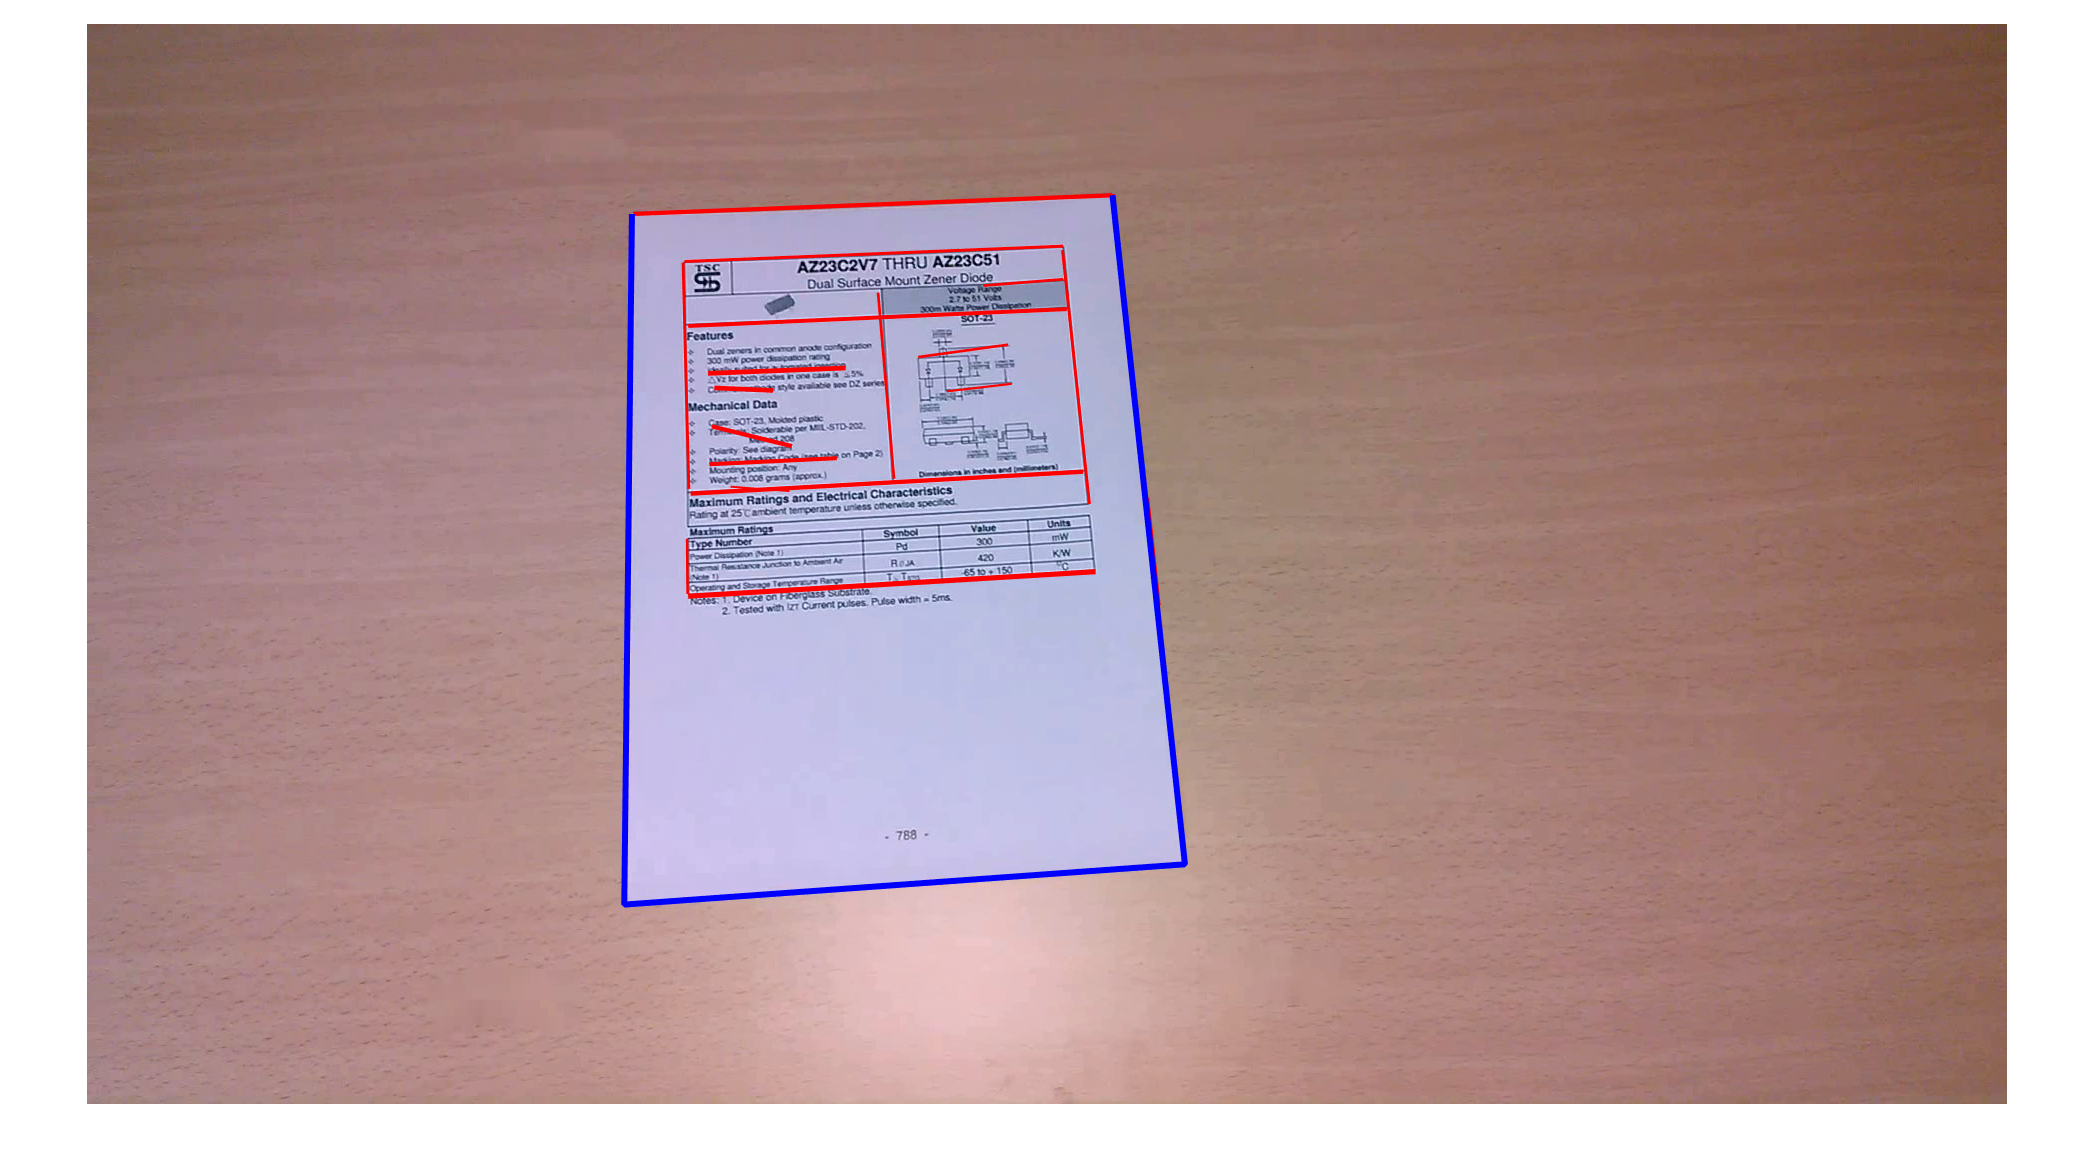
\includegraphics[width=0.7\textwidth]{bb.png}
\caption{Bounding box in blue of the document.}
\label{fig:bb}
\end{figure}

\subsection{Frame Interpolation}
If we get no bounding box from the algorithm or the bounding box is smaller than the average bounding boxes in the complete video we interpolate between frames with areas that have an area greater than the average area of the bounding boxes.

\section{Performance}
One big drawback of the algorithm is the execution time that depends on the number of founded line segments. We calculate for every combination of two horizontal and two vertical lines a bounding box. This is huge expense even with a small number of lines due to the permutations. Another problem is that the LSD algorithm takes only an input image path as input. So we have to create an image for every frame and write it out.

\section{Evaluation}
To measure the performance the Jacard index measure \cite{everingham2010pascal} is used. 
The Jacard index is the intersection of the detected bounding box with the ground truth document bounding box divided through the union of the bounding boxes (see equation \ref{eq:1}).
\begin{equation}\label{eq:1}
JI(frame)= \frac{area(G\cap S))}{area(G\cup S))}
\end{equation}

The score for one video is the average of the frame scores, and the overall accuracy of the implemented method is average of all videos with different backgrounds.

\section{Results}
First, the image is converted in a gray value image. Then we use the canny edge detector with a sigma of 3 to create a binary image of the document. We chose the canny detector because it found most of the edges in the document frames, unlike Sobel or Prewitt. However, there were many distortions on the edges, so we increased the sigma from $\sqrt{2}$ to 4 to smooth the image a bit. The result of the preprocessing steps looks like Figure \ref{fig:pre}.

\begin{figure}[h]
\centering
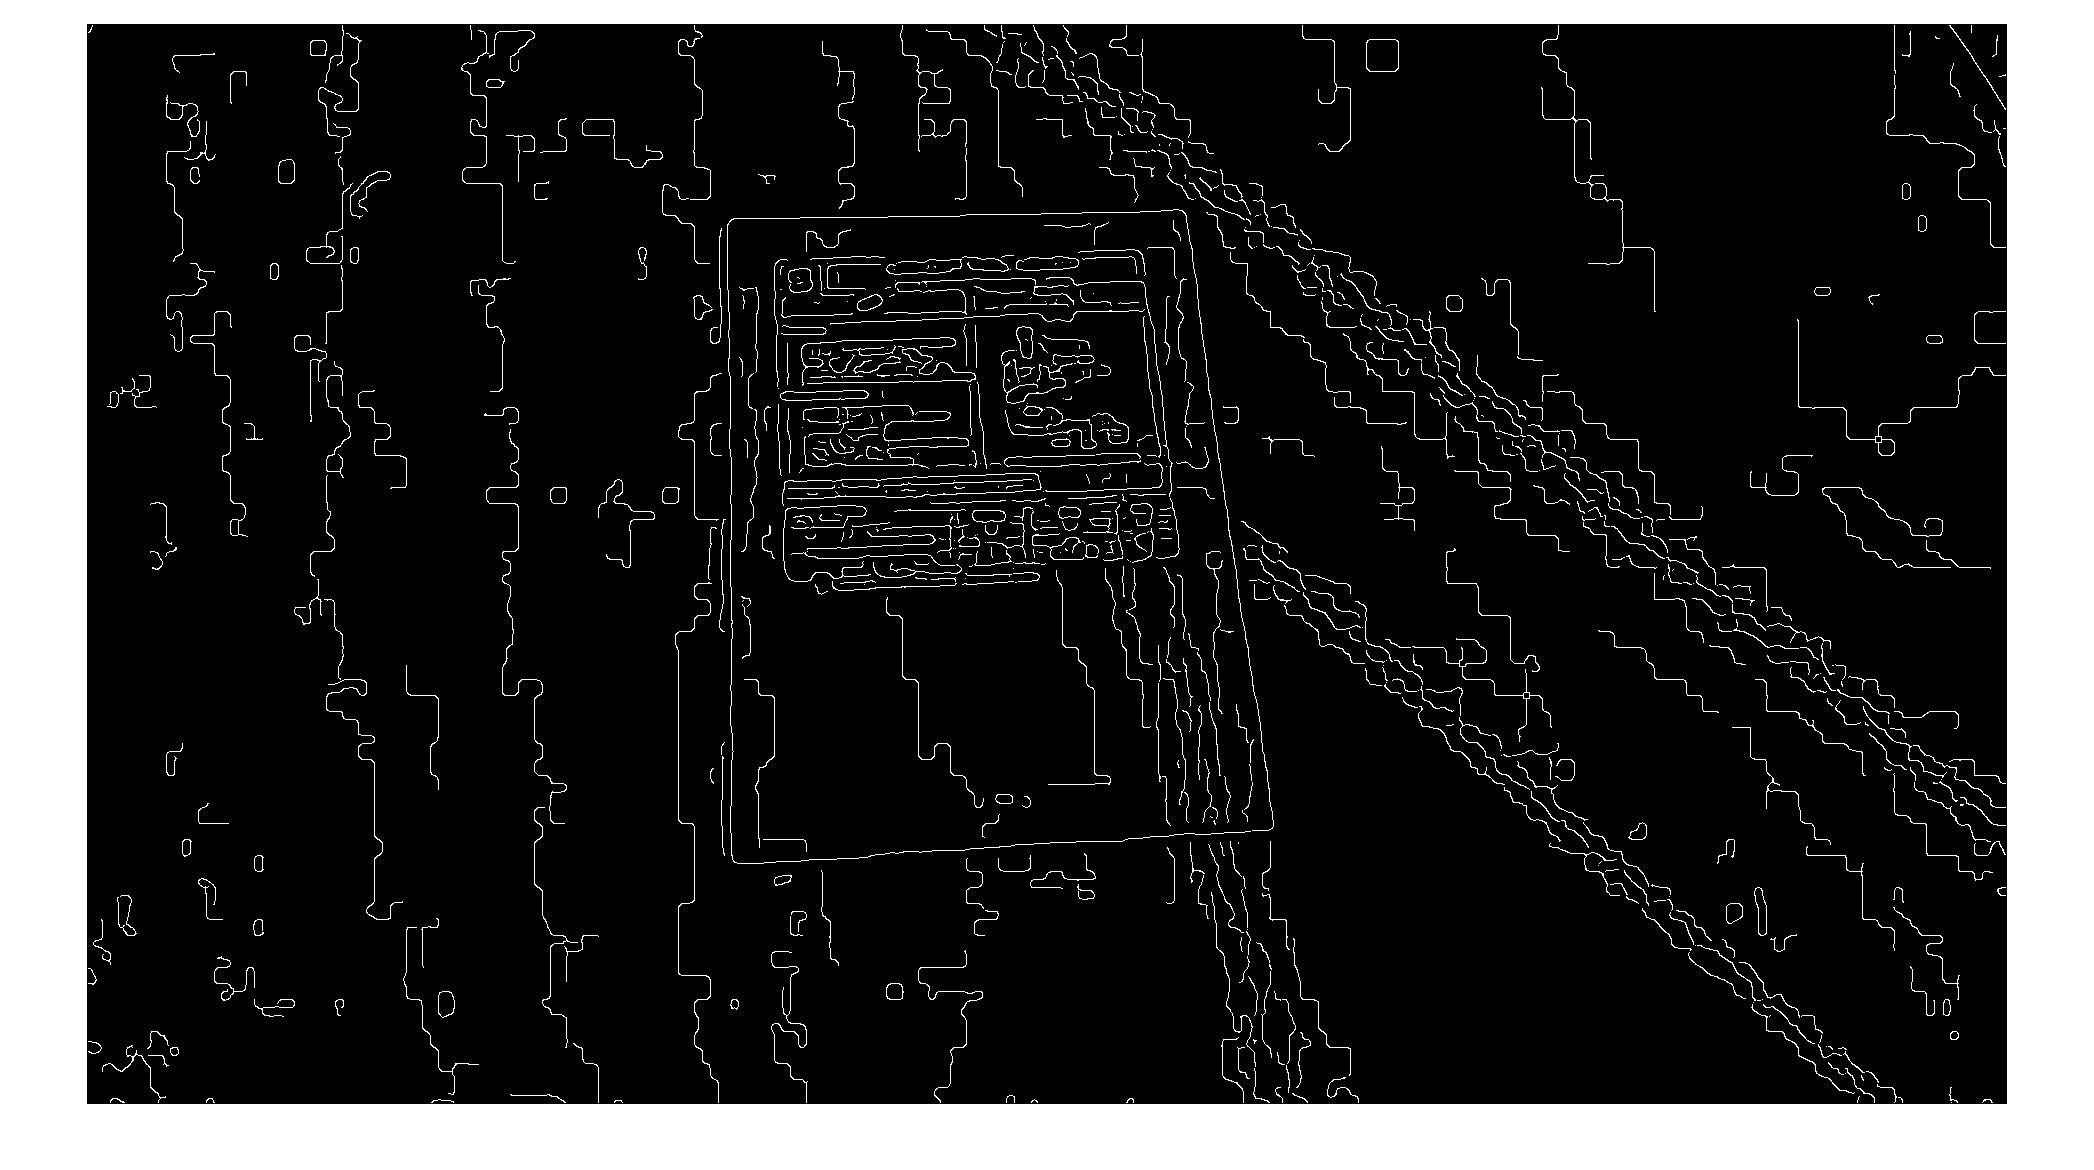
\includegraphics[width=0.7\textwidth]{pre.png}
\caption{Document frame of the image after the preprocessing step.}
\label{fig:pre}
\end{figure}

\begin{table*}[]
\centering
\caption{Jacard Index Results}
\label{tax}
\begin{tabular}{l | p{2cm}| p{2cm}| p{2cm}| p{2cm}| p{2cm} }
\hline
& \multicolumn{5}{|c}{\textbf{Background}} \\
\textbf{Document Type} &  \multicolumn{1}{c}{01} & \multicolumn{1}{c}{02} & \multicolumn{1}{c}{03} & \multicolumn{1}{c}{04} &\multicolumn{1}{c}{05} \\ \hline\hline
Datasheet & 0.961804   & 0.933321  &0.956437 &0.338121 &0.419252  \\ 
           &0.969550 & 0.949776  &0.953702 &0.670783 &0.204255  \\ 
           & 0.958112  & 0.926158  &0.954332 &0.460790 &0.407288  \\ 
           & 0.963166  & 0.942556  &0.957530 &0.406976 &0.279959  \\ 
           & 0.956819  & 0.931061  &0.964136 &0.480986 &0.373999  \\ \hline
Letter & 0.966585 & 0.931361  &0.964660 &0.548722 &0.488031  \\    
		& 0.962465 & 0.950924  &0.939243 &0.637083 &0.454185  \\ 
		& 0.962962 & 0.943569  &0.901809 &0.444535 &0.463177  \\ 
		& 0.955535 & 0.945724  &0.939415 &0.690977 &0.405386  \\ 
		& 0.959804 & 0.939154  &0.941210 &0.414960 &0.624913  \\ \hline 
Magazine & 0.961872 & 0.906609  &0.945897 &0.169548 &0.042877  \\   
		& 0.959672 & 0.937086  &0.919084 &0.148990 &0.110548  \\ 
		& 0.922668 & 0.900296  &0.941420 &0.693086 &0.000000  \\ 
		& 0.886081 & 0.863409  &0.915656 &0.389279 &0.552460  \\ 
		& 0.922554 & 0.813186  &0.964260 &0.458704 &0.175053  \\ \hline 	
Paper & 0.956659 & 0.967295  &0.952133 &0.667463 &0.410692  \\   
		& 0.954750 & 0.959377  &0.904080 &0.610046 &0.015565  \\ 
		& 0.943191 & 0.955013  &0.950578 &0.557951 &0.408258  \\ 
		& 0.923238 & 0.947480  &0.971184 &0.643748 &0.447700  \\ 
		& 0.954222 & 0.934069  &0.962020 &0.614676 &0.453615  \\ \hline 	
Patent & 0.944150 & 0.950614  &0.915164 &0.629440 &0.464737  \\   
		& 0.934623 & 0.942731  &0.906549 &0.634424 &0.380177  \\ 
		& 0.939969 & 0.935944  &0.956033 &0.538994 &0.502359  \\ 
		& 0.944970 & 0.918508  &0.897266 &0.226930 &0.358804  \\ 
		& 0.914572 & 0.837318  &0.954834 &0.548980 &0.311188  \\ \hline 
Tax & 0.949686 & 0.902505  &0.944010 &0.342882 &0.490883  \\   
		& 0.940098 & 0.937493  &0.956152 &0.575945 &0.016099  \\ 
		& 0.867588 & 0.938492  &0.933569 &0.466925 &0.062252  \\ 
		& 0.903321 & 0.880571  &0.936461 &0.419935 &0.047539  \\ 
		& 0.951203 & 0.932429  &0.930931 &0.249198 &0.500233  \\ 	\hline \hline 
\textbf{Overall/Background} &0.9431 & 0.9251 & 0.9410 & 0.4894 &0.3290\\ \hline 
\textbf{Overall}&	 0.7255					            
\end{tabular}
\end{table*}

\newpage
\bibliographystyle{plain}
\bibliography{lit}
%% References can be stored in a seperate bib-file (see lit.bib). References, that are cited in the report using \cite are automatically added to the reference list. For more information: http://www.bibtex.org/Using/
%%------------------------------------------------------
\end{document}
